

%% -*- LaTeX -*- This is LaTeX2e code

\section{Space-Efficient Tools} \label{sec:tools}
In this section, we outline a number of tools that will be useful in the sequel.

\subsection{Space-Efficient Divide-and-Conquer}\label{sec:dc}


In this subsection, we describe a simple scheme for space-efficiently
performing divide-and-conquer. In a standard recursive procedure, prior to each
recursive call, the current state of the procedure (i.e. the state of the
variables, program counter, etc.)  that is invoking the recursive call
is saved on a stack.  The variables making up the current state are
often referred to as the {\em activation frame} and the stack is
usually called the {\em recursion stack}. According to our model, a
constant amount of memory is sufficient to store one activation frame on
the recursion stack. Thus, in the standard recursive approach, the
amount of extra space needed for the recursion stack is directly
related to the height of the recursion tree.

In most divide-and-conquer situations, the recursion tree is balanced,
implying that only \Oh{\log n} extra space is needed for maintaining
the recursion stack when the input has size $n$.  In randomized
algorithms, such as Quicksort, the recursion tree can have linear
height in the worst case. However, by always recursing on the smaller
sub-array first\footnote{This is sometimes referred to as optimizing
tail recursion.}, a worst case size of \Oh{\log n} for the stack can
be maintained\cite{huang:one-way,wegner:generalized}.  Consider
Algorithm \ref{alg:recurse} below, which represents a generic template
for divide-and-conquer algorithms.  Note that ``PROCESS x" simply
refers to a set of non-recursive statements.


\begin{algorithm}
  \caption{\textsc{Recursive}($b,e$): Standard template for recursion}
  \label{alg:recurse}
  \begin{algorithmic}[1]
    \IF{$e-b < s$ where $s$ is the size of the recursion base.}
    \STATE \{PROCESS 1: Base instance operations.\}
    \ELSE
    \STATE \{PROCESS 2: Computations to partition the array $A[b,\ldots,e-1]$\}
    \STATE \textsc{Recursive}($b,\lfloor e/2 \rfloor$)
    \STATE \textsc{Recursive}($\lfloor e/2 \rfloor + 1,e$)
    \STATE \{PROCESS 3: Pre-merge operations\}
    \STATE Merge $A[b,\lfloor e/2 \rfloor-1]$ with $A[\lfloor e/2
\rfloor + 1,e-1]$.
    \STATE \{PROCESS 4: Post-merge operations\}
    \ENDIF
  \end{algorithmic}
\end{algorithm}

Can a balanced recursion tree arising from the above recursive
algorithm be traversed with only \Oh{1} extra memory as opposed to the
\Oh{\log n} extra memory used for the stack?  Our technique outlines a
method for converting any algorithm fitting the above recursive
template into one that uses only \Oh{1} extra memory. The recursion
tree is traversed in the same manner without use of the recursion
stack. In many cases, the same type of result can be obtained using
bottom-up merge, however, it is well known that bottom-up merge has
poor performance in the presence of caches.

The main idea (which is probably folklore, even though we have not
seen it explicitly in the literature) is to simulate a post-order
traversal of the recursion tree. We assume for simplicity that the
data to be processed is stored in an array $A=A[0,\ldots,n-1]$ of size
$n = 2^k$ for some positive integer $k$. The recursion tree
corresponding to the above divide-and-conquer scheme is a perfectly
balanced binary tree, in which each node at depth $0 \leq i < k$
corresponds to a subarray of the form $A[j \cdot 2^{k-i} ,\ldots, (j +
1) \cdot 2^{k-i} - 1]$ for some integer $0 \leq j \leq i$.\footnote{If
the problem size is not an exact power of two, we imagine the
recursion tree to be embedded into a perfectly balanced tree and stop
traversing the tree prematurely.}

Our scheme is presented in Algorithm~\ref{alg:traversal}. We maintain
two indices $b$ and $e$ that indicate the subarray $A[b ,\ldots, e-1]$
currently processed. We will use the binary representation of the
index $e$ to implicitly store the current status of the post-order
traversal, i.e., the node of the simulated recursion tree currently
visited.

\begin{algorithm}
  \caption{$\textsc{Stackless-Recursive}(b,e)$: Stackless simulation
of \textsc{Recursive}}
  \label{alg:traversal}
  \begin{algorithmic}[1]
    \STATE $b=0$ and $e=s$, $s$ is the size of the recursion base.
    \WHILE{$b\neq 0$ or $e\leq n$}
    \STATE \{PROCESS 1: Base instance operations. Process all items in
$A[b,\ldots, e-1]$.\}
    \STATE $i$ be the index of the least significant bit of $e$.
    \FOR{$c\gets 1,\ldots, i$}
    \STATE $b \gets e-2^c$.
    \STATE \{PROCESS 3: Pre-merge operations\}
    \STATE Merge  $A[b,\ldots, b+2^{c-1} - 1]$ with
$A[b+2^{c-1},\ldots, e-1]$
    \STATE \{PROCESS 4: Post-merge operations on $A[b,\ldots, e-1]$ \}
    \ENDFOR 
    %\STATE $b \gets e$.  Not needed because of line 7.
    \STATE $e \gets e + s$.
    \ENDWHILE
  \end{algorithmic}
\end{algorithm}

Determining the value of $i$ (Step 4) can be done in \Oh{1} amortized
time without extra space using a straightforward implementation of a
binary counter.  The above algorithm basically traverses the recursion
tree from left to right. When processing a leaf $v$, the algorithm
backtracks in geometrically increasing steps merging all subtrees
already traversed completely. This merging is done by traversing a
leaf-to-root path starting from $v$ but stopping as soon as the path
goes up to the right (Figure~\ref{fig:tree_spaceefficient}). The
correctness of the algorithm follows from the next
lemma\cite{cormen:alg}:

\begin{lemma}
  If the leaves of a complete binary tree are labeled from left to
  right (starting with $1$ for the leftmost leaf), the height of the
  largest subtree containing the leaf $e>1$ as its rightmost leaf is
  equal to the index $i$ of the least significant bit of the number
  $e$.
\end{lemma}

\begin{figure}
  \centerline{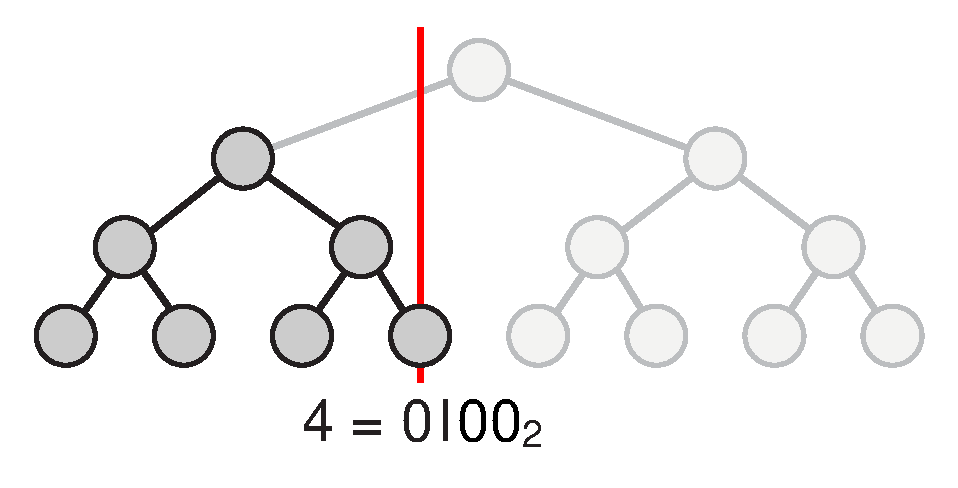
\includegraphics[height=3.5cm]{tree_spaceefficient}}
  \caption{Merging subtrees while traversing left-to-right.}
  \label{fig:tree_spaceefficient}
\end{figure}

Therefore, any algorithm that is in the form outlined by Algorithm
\ref{alg:recurse} using \Oh{\log n} extra space can be transformed
into a space-efficient algorithm of the form Algorithm \ref{alg:traversal}
using only \Oh{1} extra space provided that all the base instances
(i.e. leaves of the recursion tree) can be pre-computed with only \Oh{1} extra
space and PROCESS 1,3,4 as well as the Merge step can be made
space efficient using only \Oh{1} extra space. Note that PROCESS 2
operations no longer need to be computed in Algorithm \ref{alg:traversal}
since we assume that the array is initially partitioned into the
base instances. Therefore, there is no need to actually partition
the array as is done in PROCESS 2 in Algorithm \ref{alg:recurse}. Henceforth, we will refer
to recursive algorithms in standard form (i.e. Algorithm
\ref{alg:recurse}) as the {\em standard recursive form} and
space-efficient recursive algorithms (i.e. Algorithm \ref{alg:traversal})
as {\em space-efficient recursive form}. We conclude this section
with the following:

\begin{theorem}
An algorithm in standard recursive form running in \Oh{n \log n} time and using \Oh{\log n} extra space can be converted
to space-efficient recursive form running in \Oh{n \log n} time using only \Oh{1} extra space provided that all the base instances
(i.e. leaves of the recursion tree) can be pre-computed in \Oh{n \log n} time with only \Oh{1} extra
space and PROCESS 1,3,4 as well as the Merge step can be made
space efficient using only \Oh{1} extra space and \Oh{n} time.
\end{theorem}

Note that there can be trade-offs in the above theorem. For example, if in the space-efficient recursive form, the Merge step takes
\Oh{n \log n} time then, the overall running time becomes \Oh{n \log^2 n}. These trade-offs are fairly straightforward, related to the
Master Theorem for Recurrences \cite{cormen:alg} and can be adjusted to each situation.

\subsection{Sorted Subset Selection}

In this subsection, we introduce a simple yet surprisingly powerful
algorithm, called \textsc{SortedSubsetSelection}$(A,b,e,f)$.  The
algorithm provides a way of stably selecting a subset of the elements.
The key requirement is that the elements stored in the given array
$A[b,\ldots, e-1]$ are initially sorted according to some total order,
say $<_{A}$. The algorithm, described below as
Algorithm~\ref{alg:sortedSubsetSelection}, stably moves to the front
of the array all elements in $A[b,\ldots, e-1]$ for which the given
$(0,1)$-valued function $f$ returns the value one.  Moreover, this
algorithm has the desirable property that its effect can be reversed
easily.

\begin{algorithm}
  \caption{Algorithm
    $\textsc{SortedSubsetSelection}(A,b,e,f)$ for selecting a
    subset from a sorted array $A[b,\ldots, e-1]$.} 
  \label{alg:sortedSubsetSelection}
  \begin{algorithmic}[1]
    \REQUIRE Array $A[b,\ldots, e-1]$ is sorted according to
    some total order $<_{A}$, and $f$ is a 
    $(0,1)$-valued function that can be evaluated in constant
    time.
    
    \ENSURE $A[b,\ldots, m-1]$ contains all entries for which
    $f$ is one, and these entries are still (stably) ordered
    according to $<_{A}$.

    \STATE $i\gets b$, $j\gets b$ and $m\gets b+1$. 
    \WHILE{$i<e$ and $j<e$}
      \WHILE{$i<e$ and $f(A[i])=1$}
        \STATE $i\gets i+1$. \COMMENT{Move index $i$ such that
          $f(A[i])=0$.} 
      \ENDWHILE
      \STATE $j\gets i+1$;
      \WHILE{$(j<e)$ and $(f(A[j])=0)$}
        \STATE $j\gets j+1$. \COMMENT{Move index $j$ such that
        $f(A[j])=1$.} 
      \ENDWHILE
      \IF{$j<e$}
        \STATE Swap $A[i]$ and $A[j]$.
        \STATE $m\gets i+1$. \COMMENT{$A[b,\ldots, m-1]$
          contains all 1-valued entries.}
      \ENDIF
    \ENDWHILE
    \STATE Return $m$.
  \end{algorithmic}
\end{algorithm}

Algorithm~\ref{alg:sortedSubsetSelection} clearly uses only \Oh{1}
extra space and runs in linear time. The correctness of the algorithm
follows from the loop invariant that is maintained: $A[b,\ldots, m-1]$
stably contains all selected elements from $A[b,\ldots, e-1]$ whose rank
is at most $m-b$.  The effects of this algorithm can be reversed by
Algorithm~\ref{alg:revertSortedSubsetSelection}.

\begin{algorithm}
  \caption{Algorithm $\textsc{UndoSubsetSelection}(A,b,e,m)$
    for restoring the total order after applying the 
    \textsc{SortedSubsetSelection}-Algorithm~\ref{alg:sortedSubsetSelection}}
  \label{alg:revertSortedSubsetSelection}
  \begin{algorithmic}[1]

    \REQUIRE{Array $A[b,\ldots, m-1]$ contains the result of running
      Algorithm~\ref{alg:sortedSubsetSelection} on array
      $A[b,\ldots, e-1]$ that was sorted according to
      $<_{A}$.} 
    \ENSURE{Array $A[b,\ldots, e-1]$ is sorted according to
      $<_{A}$.} 
    \STATE $i\gets m-1$ and $j\gets e-1$.
    \WHILE{$i\neq j$ and $i\geq b$}
      \IF{$A[j]<_{A}A[i]$}
        \STATE Swap $A[i]$ and $A[j]$.
        \STATE $j\gets j-1$.
      \ENDIF
      \STATE $i\gets i-1$.
    \ENDWHILE

  \end{algorithmic}
\end{algorithm}

There is one important property to note:
Algorithm~\ref{alg:revertSortedSubsetSelection} does not require
knowledge of the selection function $f$, but only needs to know the
three indices $b$, $e$ and $m$. It only uses the order $<_{A}$ to
recover the state prior to the invocation of
\textsc{SortedSubsetSelection}. This is a key property that is useful
particularly if the selection function $f$ is unknown or cannot be
easily reconstructed.  In the following subsection, we show how useful
\textsc{SortedSubsetSelection} and its counterpart
\textsc{UndoSubsetSelection} are.


\subsection{Selecting the $k$-th smallest element}\label{sec:sel}

Selection of the $k$-th smallest element in-place is a fairly
difficult problem which makes use of stable partition which is
notoriously complicated\cite{kata:select}. However, in most geometric problems,
the input consists of a set of points in 2 or more dimensions.  If
the points are sorted with respect to one coordinate, selection of
the $k$-th smallest element with respect to another coordinate
becomes much easier.  We can take advantage of the total order in
one coordinate to simplify selection through the use of
SortedSubsetSelection. We outline a simple randomized algorithm
that runs in linear expected time and uses only \Oh{1} extra space.
Our algorithm is a slight modification of QuickSelect\cite{hoare:quicksort, cormen:alg}.


\begin{algorithm}
  \caption{Algorithm
    $\textsc{Select}(A,0,e,k)$ Select element in $A[0,e-1]$ with $k$-th smallest $X$-coordinate.}

  \label{alg:selectk}
  \begin{algorithmic}[1]
    \REQUIRE Array $A[0,\ldots, e-1]$ is sorted according to $Y$-coordinate.
    
    \ENSURE Element with $k$-th smallest $X$-coordinate is placed at
$A[0]$, and $A[1,\ldots, e-1]$ is sorted by $Y$-coordinate.

    \STATE $n \gets e$. \COMMENT{$n$ is the current size of the array being processed. }
    \WHILE{$n > 42$}
          \IF{k $< n/2$}
             \STATE Pick a random element $x$ whose rank is between $n/2$ and $3n/4$.
             \STATE Use \textsc{SortedSubsetSelection} to move all elements $< x$ and a sufficient number $> x$ to fill $A[0,\lfloor 3n/4 \rfloor - 1]$.
             \STATE Push $4(3n/4 - \lfloor 3n/4 \rfloor)$ on stack S.
             \STATE $n \gets \lfloor 3n/4 \rfloor$
          \ELSE
             \STATE Pick a random element $x$ whose rank is between $n/4$ and $n/2$.
             \STATE Use \textsc{SortedSubsetSelection} to move all elements $> x$ and a sufficient number $< x$ to fill $A[0,\lfloor 3n/4 \rfloor - 1]$.
             \STATE Push $4(3n/4 - \lfloor 3n/4 \rfloor)$ on stack S.
             \STATE $k \gets k - \lceil n/4 \rceil$.
             \STATE $n \gets \lfloor 3n/4 \rfloor$
          \ENDIF
    \ENDWHILE
    \STATE Find $k$-th smallest element in A[0,n-1] by brute force. $K
\gets$ this element.
    \STATE $M \gets n$
    \STATE $R \gets$ Pop top of stack.
    \STATE $D \gets (4M + R)/3$.
    \WHILE{$D < e$}
          \STATE UndoSubsetSelection($A,0,D,M$)
          \STATE $M \gets D$.
          \STATE $R \gets$ Pop top of stack.
          \STATE $D \gets (4M + R)/3$.
    \ENDWHILE
    \STATE Find $K$ in A[$0,\ldots, e-1$] and move it stably to A[$0$].
  \end{algorithmic}
\end{algorithm}

The main idea behind the algorithm is fairly simple. Refer to
Algorithm~\ref{alg:selectk}. If $k$ is smaller than $n/2$, then we
find an element $x$ whose rank is between $n/2$ and $3n/4$. The case
is similar if $k \geq n/2$. Since there are at least $n/4$ such
elements, with only an expected constant number of random selections,
we can find such an element.  Computing the rank of a given element
takes \Oh{n} time, thus in \Oh{n} expected time, we can find $x$. Note
that if we partition the array with $x$, then at least $n/4$ elements
can be eliminated.  The key is to eliminate {\em precisely} $n/4$
elements. This way, when it comes time to undo the operation, we know
exactly where the partition boundaries occur. This is where the stack
$S$ comes into play.  Each time through the loop, we reduce the size
of the array to $\lfloor 3n/4 \rfloor$. To undo this operation, we
need to record the actual remainder from the division by $3/4$. Two
bits are sufficient to record this since the remainder can only be one
of $\{0, 1, 2, 3\}$.  For example, suppose that the current instance
has an array of size 37.  Since $3\times 37/4 = 27+3/4$, the next
instance has size $27$ and we push the remainder $3$ on the stack.  In
the undo step, if the current instance is 27, to recover the size of
the array at invocation, we note that $(4*27 + 3)/3 = 37$ which is the
computation used to recover the indices required for the Undo
operation.

In the final loop where the steps are {\em undone}, the only
information we require are the three indices $0, D$ and $M$. We do not
need to remember the particular element $x$ that was used in the SortedSubsetSelection step. 
The sorted order on the $Y$-coordinate
is sufficient to recover the original order. 

Since at each iteration through the while loop, we eliminate
a quarter of the elements, the number of iterations through the loop is \Oh{\log n}. At
each iteration, two bits are pushed on the stack, so the total number of bits ever
stored in the stack is \Oh{\log n} which implies that only \Oh{1} extra space
is used. The running time of the algorithm is given by the following recurrence:
\[
T(n) = T(3n/4) + \Oh{n}
\] 
which resolves to \Oh{n}.

This algorithm can be made \Oh{n} deterministic. The only step where randomization is used is in the selection 
of the partition element $x$. In the deterministic version, we use techniques from 
the algorithm by Blum \etal~\cite{blum:selection}.
Instead of selecting an element at random, we select the partition element by first decomposing the
array into $n/5$ groups of 5 elements and computing the median of the medians of the groups. 
The idea is simple and similar to the above algorithm except some of the details are quite tedious, so we outline the details
in Appendix \ref{sec:detkmed}.





%%% Local Variables:
%%% mode: latex
%%% TeX-master: "paper"
%%% End:
